% ==========================================
% BAB V IMPLEMENTASI
% ==========================================
\cleardoublepage
\chapter{IMPLEMENTASI SISTEM}
\label{chap:implementasi-sistem}

Bab ini memaparkan hasil implementasi dari perancangan sistem yang telah diuraikan pada bab sebelumnya. 
Fokus pembahasan mencakup realisasi antarmuka pengguna (\textit{frontend}) beresolusi tinggi (\textit{high-fidelity}), 
implementasi mekanisme autentikasi dan proteksi rute, integrasi antarmuka dengan layanan \textit{backend} melalui 
REST API, penanganan kondisi data tidak normal, serta konfigurasi aplikasi sebagai \textit{Progressive Web App} (PWA).

\section{Tumpukan Teknologi Frontend}

\textit{Frontend} pada tugas akhir ini dikembangkan menggunakan Next.js \autocite{vercel_nextjs} sebagai \textit{framework}
utama dengan dukungan TypeScript dan TanStack Query \autocite{linsley_tanstack}. Alasan pemilihan ketiga teknologi
tersebut dibandingkan dengan alternatifnya telah diuraikan pada Bab~\ref{chap:analisis-masalah}. Subbab ini
menjelaskan peran konkret masing-masing teknologi dalam implementasi \textit{frontend dashboard} yang dibangun.

\subsection{Next.js}

Pada tugas akhir ini, Next.js digunakan sebagai fondasi \textit{frontend dashboard
monitoring}. \textit{Framework} ini bertanggung jawab terhadap navigasi antarhalaman,
pengelolaan layout, pemuatan halaman, serta integrasi berbagai komponen yang
digunakan untuk membangun antarmuka operator.

\subsection{TypeScript}

Dalam tugas akhir ini, TypeScript digunakan untuk mendefinisikan model data,
respons API, parameter fungsi, serta properti komponen. Penggunaan TypeScript
membantu meningkatkan keterbacaan kode, mempermudah proses pemeliharaan, serta
mengurangi potensi kesalahan selama pengembangan frontend.

\subsection{TanStack Query}

Pada frontend dashboard WTP, TanStack Query digunakan untuk mengambil data
sensor, ringkasan kepatuhan, alarm, riwayat pengukuran, status pompa, level
tangki bahan kimia, serta informasi operasional lainnya melalui REST API.
Penggunaan TanStack Query juga menyederhanakan pengelolaan proses
\textit{loading}, pembaruan data, dan sinkronisasi informasi pada berbagai
halaman dashboard.

\section{Implementasi Antarmuka Pengguna}
Implementasi antarmuka pengguna merupakan tahap transformasi dari purwarupa \textit{low-fidelity} menjadi antarmuka
interaktif yang berjalan di atas peramban web. Antarmuka ini dibangun menggunakan komponen-komponen React yang dikelola 
melalui \textit{framework} Next.js dengan bahasa pemrograman TypeScript.

\subsection{Halaman \textit{Dashboard} Utama}
Halaman \textit{dashboard} utama merupakan titik pusat pemantauan operasional \textit{Water Treatment Plant} (WTP). Halaman 
ini dirancang untuk menyajikan rangkuman kondisi keseluruhan pabrik agar operator dapat mengambil keputusan secara cepat dan tepat. 
Hasil implementasi halaman \textit{dashboard} ditunjukkan pada Gambar~\ref{fig:hifi-dashboard}.

\begin{figure}[htbp]
    \centering
    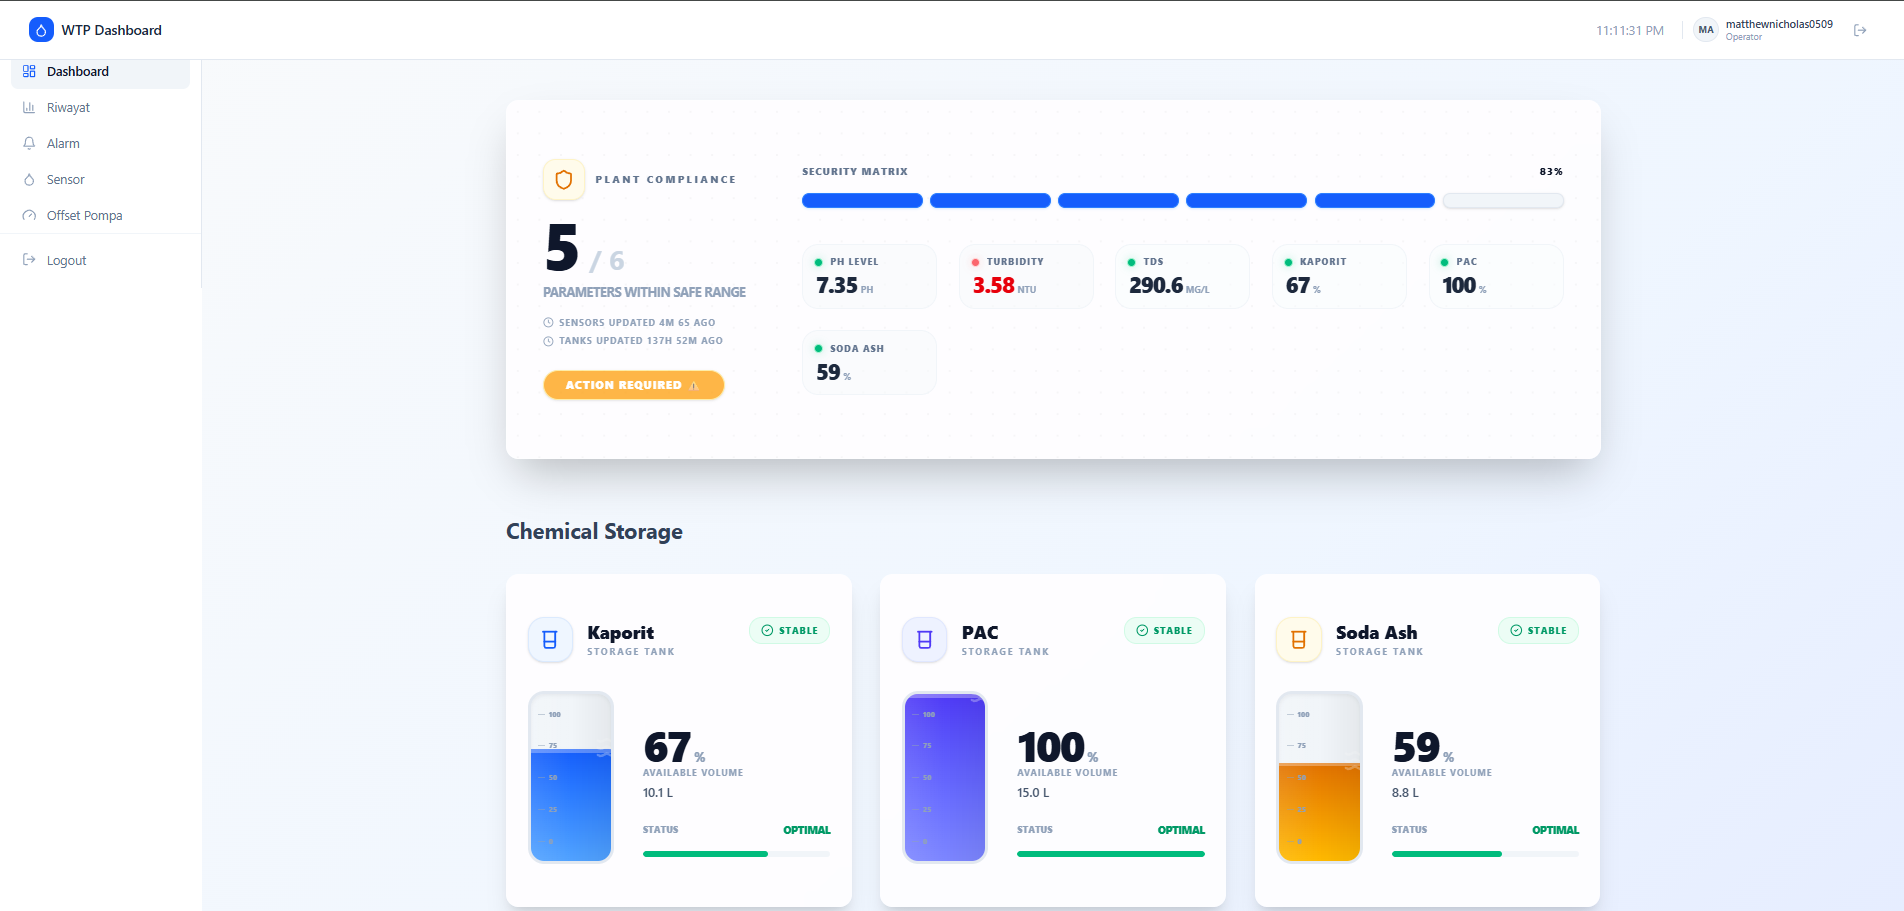
\includegraphics[width=\textwidth]{images/dash-hifi.png} 
    \caption{Implementasi antarmuka halaman \textit{dashboard} utama}
    \label{fig:hifi-dashboard}
\end{figure}

Berdasarkan Gambar~\ref{fig:hifi-dashboard}, tata letak halaman telah diimplementasikan sesuai dengan rancangan purwarupa. 
Struktur antarmuka dibagi menjadi beberapa komponen fungsional utama:
\begin{enumerate}
    \item \textbf{Panel Navigasi (\textit{Sidebar}) dan \textit{Header}:} 
    Terletak di sisi kiri, \textit{sidebar} memuat menu navigasi utama aplikasi (Dashboard, Riwayat, Alarm, Sensor, Offset 
    Pompa, dan Logout). Pada bagian atas (\textit{header}), terdapat informasi waktu sistem dan identitas profil operator 
    yang sedang aktif beserta perannya.

    \item \textbf{Panel Kepatuhan Sistem (\textit{Plant Compliance}):}
    Komponen \texttt{ComplianceSummary} bertindak sebagai indikator kesehatan utama WTP. Sistem menampilkan metrik 
    jumlah parameter yang berada dalam batas aman (ditampilkan sebagai $5/6$ \textit{Parameters Within Safe Range}) 
    beserta persentase kepatuhannya. Panel ini juga merangkum nilai pembacaan telemetri terkini, seperti pH air (7,35), 
    kekeruhan (3,58 NTU), \textit{Total Dissolved Solids} atau TDS (290,6 mg/L), serta persentase stok bahan kimia 
    untuk kaporit, PAC, dan soda ash. Selain itu, ditampilkan pula penanda waktu pembaruan terakhir data sensor maupun 
    data tangki sehingga operator dapat menilai kesegaran (\textit{freshness}) informasi yang sedang dilihat.

    \item \textbf{Visualisasi Penyimpanan Bahan Kimia (\textit{Chemical Storage}):}
    Komponen \texttt{ChemicalTank} menampilkan tiga kartu (\textit{cards}) untuk tangki kaporit, 
    \textit{Polyaluminium Chloride} (PAC), dan soda ash. Representasi visual ketinggian cairan di dalam masing-masing 
    tangki diimplementasikan secara dinamis menggunakan manipulasi \textit{Cascading Style Sheets} (CSS) yang nilainya 
    diikat (\textit{binding}) langsung dengan persentase data dari API (misalnya PAC terisi 100\% dengan volume tersedia 
    15 L). Setiap kartu juga dilengkapi indikator status ketersediaan bahan kimia yang ditentukan berdasarkan nilai 
    ambang batas yang dikirimkan melalui respons ringkasan \textit{dashboard}.

    \item \textbf{Status Pompa Injeksi (\textit{Pump Status}):}
    Terletak di area bawah halaman, komponen ini menampilkan status operasional (\textit{on/off}) dari masing-masing 
    pompa aktuator bahan kimia secara sekilassehingga operator dapat mengamati ketersediaan bahan kimia dan aktivitas 
    pompa dari layar pemantauan yang sama.
\end{enumerate}

\subsection{Halaman Riwayat Sensor}
Halaman riwayat sensor (\textit{Data History}) diimplementasikan sebagai modul peninjauan historis 
pada \textit{frontend}. Halaman ini memfasilitasi operator untuk melakukan peninjauan tren kualitas air secara 
historis, yang krusial untuk keperluan evaluasi kinerja sistem maupun pelaporan audit lingkungan. Hasil 
implementasi halaman riwayat ditunjukkan pada Gambar~\ref{fig:hifi-history}.

\begin{figure}[htbp]
    \centering
    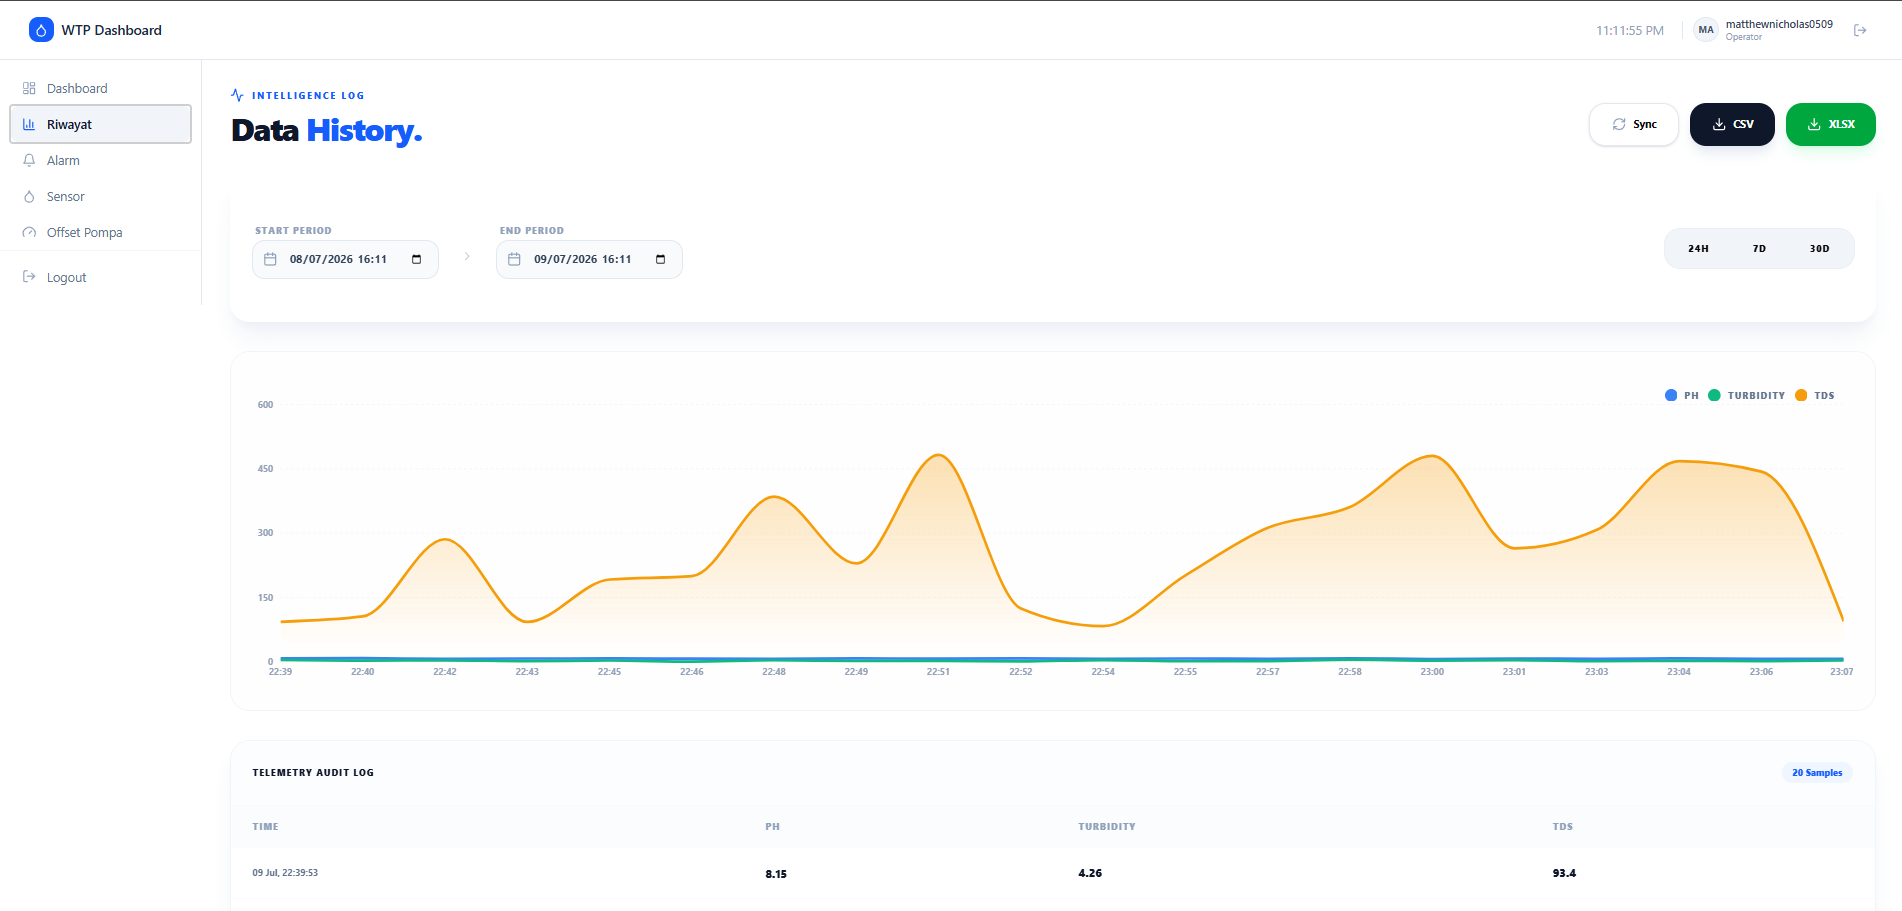
\includegraphics[width=\textwidth]{images/history-hifi.png} 
    \caption{Implementasi antarmuka halaman riwayat sensor}
    \label{fig:hifi-history}
\end{figure}

Berdasarkan Gambar~\ref{fig:hifi-history}, tata letak dan fungsionalitas halaman ini disusun untuk mendukung 
eksplorasi data telemetri dalam jumlah besar. Komponen-komponen utama yang diimplementasikan pada halaman ini meliputi:
\begin{enumerate}
    \item \textbf{Panel Penyaringan Waktu (\textit{Time Filter}):} 
    Terdapat komponen pemilih tanggal dan waktu (\textit{date/time picker}) untuk menentukan parameter \textit{Start Period} 
    dan \textit{End Period}. Selain penentuan manual, antarmuka juga menyediakan tombol pintas 
    (\textit{quick filters}) untuk mengambil rentang data 24 jam terakhir (24H), 7 hari (7D), dan 30 hari (30D). 
    Pemilihan rentang waktu ini bertindak sebagai \textit{client state} yang akan dikirimkan sebagai parameter kueri 
    (\textit{query parameter}) ke REST API.

    \item \textbf{Kontrol Sinkronisasi dan Ekspor Laporan:} 
    Di sudut kanan atas, terdapat tombol \textbf{Sync} untuk memaksa sistem melakukan penarikan ulang data 
    (\textit{manual refetch}) dari \textit{server}. Di sebelahnya, diimplementasikan fitur ekspor data historis 
    dengan pilihan format berkas \textbf{CSV} dan \textbf{XLSX}. Fitur ini memproses data JSON yang ada di 
    dalam memori antarmuka menjadi format tabular yang siap diunduhsehingga menyederhanakan tugas operator dalam 
    menyusun laporan harian atau bulanan.

    \item \textbf{Visualisasi Grafik Tren (\textit{Trend Chart}):} 
    Komponen sentral pada halaman ini adalah kanvas grafik bertipe area (\textit{area chart}). 
    Grafik ini memetakan fluktuasi tiga parameter utama secara bersamaan, yaitu pH (biru), kekeruhan 
    atau \textit{turbidity} (hijau), dan TDS (oranye) terhadap sumbu waktu. 

    \item \textbf{Log Audit Telemetri (\textit{Data Table}):} 
    Di bagian bawah grafik, disajikan komponen tabel yang merepresentasikan titik-titik data pada grafik ke dalam wujud 
    angka eksak. Tabel ini dilengkapi dengan indikator jumlah sampel data (misalnya \textit{20 Samples}). 
    Keberadaan tabel ini berfungsi sebagai instrumen validasi silang bagi operator ketika membutuhkan detail nilai parameter.
\end{enumerate}

\subsection{Halaman Pusat Alarm (\textit{Alarm Center})}
Halaman Pusat Alarm (\textit{Alarm Center}) diimplementasikan sebagai modul tanggap insiden (\textit{incident response}). 
Halaman ini bertugas menampilkan anomali ketika parameter telemetri yang dibaca oleh sensor melampaui ambang 
batas aman yang telah dikonfigurasi pada \textit{backend}. Hasil implementasi halaman ini ditunjukkan pada Gambar~\ref{fig:hifi-alarm}.

\begin{figure}[htbp]
    \centering
    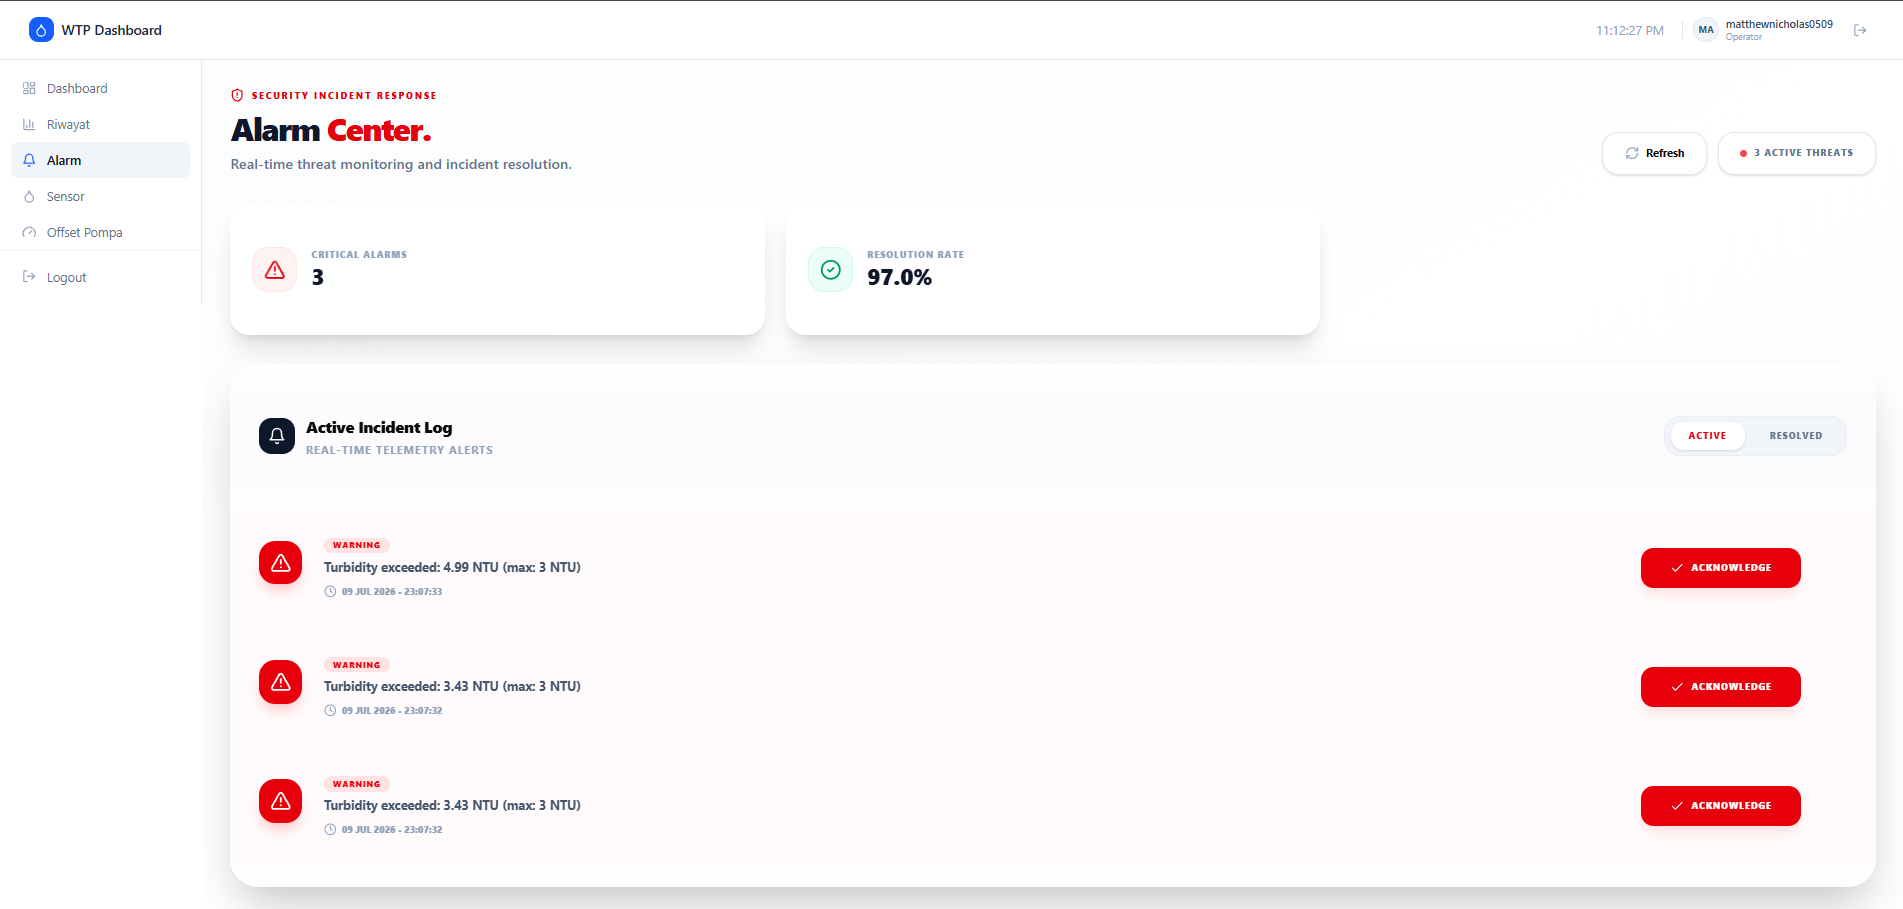
\includegraphics[width=\textwidth]{images/alarm-hifi.png} 
    \caption{Implementasi antarmuka halaman pusat alarm}
    \label{fig:hifi-alarm}
\end{figure}

Berdasarkan Gambar~\ref{fig:hifi-alarm}, antarmuka dirancang dengan mengedepankan prinsip kedaruratan visual, 
di mana warna merah kontras digunakan secara dominan untuk menarik atensi operator terhadap isu-isu kritis. 
Komponen-komponen fungsional yang diimplementasikan meliputi:
\begin{enumerate}
    \item \textbf{Indikator Metrik Resolusi (\textit{Summary Metrics}):} 
    Di bagian atas, terdapat informasi yang menampilkan jumlah alarm kritis yang sedang aktif (\textit{Critical Alarms}) 
    secara dinamis. Selain itu, terdapat indikator \textit{Resolution Rate} yang mengukur persentase historis keberhasilan operator 
    dalam menangani alarm dibandingkan dengan total alarm yang pernah terjadi.

    \item \textbf{Navigasi Status Insiden (\textit{Tab Navigation}):} 
    Pada bilah judul log insiden, diimplementasikan komponen \textit{tab switch} yang membagi data menjadi dua kategori: 
    \textbf{ACTIVE} (alarm yang belum ditangani) dan \textbf{RESOLVED} (alarm yang sudah diselesaikan). Perpindahan antartab 
    ini diatur menggunakan \textit{client state} lokal untuk memberikan transisi antarmuka yang instan tanpa memuat ulang halaman.

    \item \textbf{Daftar Log Insiden (\textit{Incident Log List}):}  
    Setiap baris mewakili satu insiden spesifik, menampilkan lencana tingkat keparahan (\textit{WARNING}), deskripsi masalah 
    beserta nilai pembacaan dan ambang batas yang terlampaui (misalnya kekeruhan terbaca 4,99 NTU terhadap batas maksimal 
    3 NTU), dan cap waktu presisi kejadian (\textit{timestamp}).

    \item \textbf{Aksi Pengakuan (\textit{Acknowledge Action}):} 
    Setiap baris alarm aktif dilengkapi dengan tombol aksi \textbf{ACKNOWLEDGE}. Ketika operator telah memeriksa kondisi 
    di lapangan dan menekan tombol ini, \textit{frontend} mengeksekusi fungsi mutasi API (\textit{API mutation}) ke 
    \textit{backend} untuk mengubah status alarm tersebut sehingga alarm berpindah 
    ke daftar \textit{resolved}.
\end{enumerate}

\subsection{Halaman Analitik Sensor}
Halaman Analitik Sensor diimplementasikan untuk memberikan tinjauan visual dan statistik yang mendalam bagi masing-masing sensor
kualitas air, yaitu sensor pH, kekeruhan (\textit{turbidity}), dan \textit{Total Dissolved Solids} (TDS). Berbeda dengan halaman 
\textit{dashboard} utama yang bersifat merangkum, halaman ini dirancang khusus untuk keperluan diagnosis parameter secara spesifik. 
Hasil implementasi antarmuka ini ditunjukkan pada Gambar~\ref{fig:hifi-sensor}.

\begin{figure}[htbp]
    \centering
    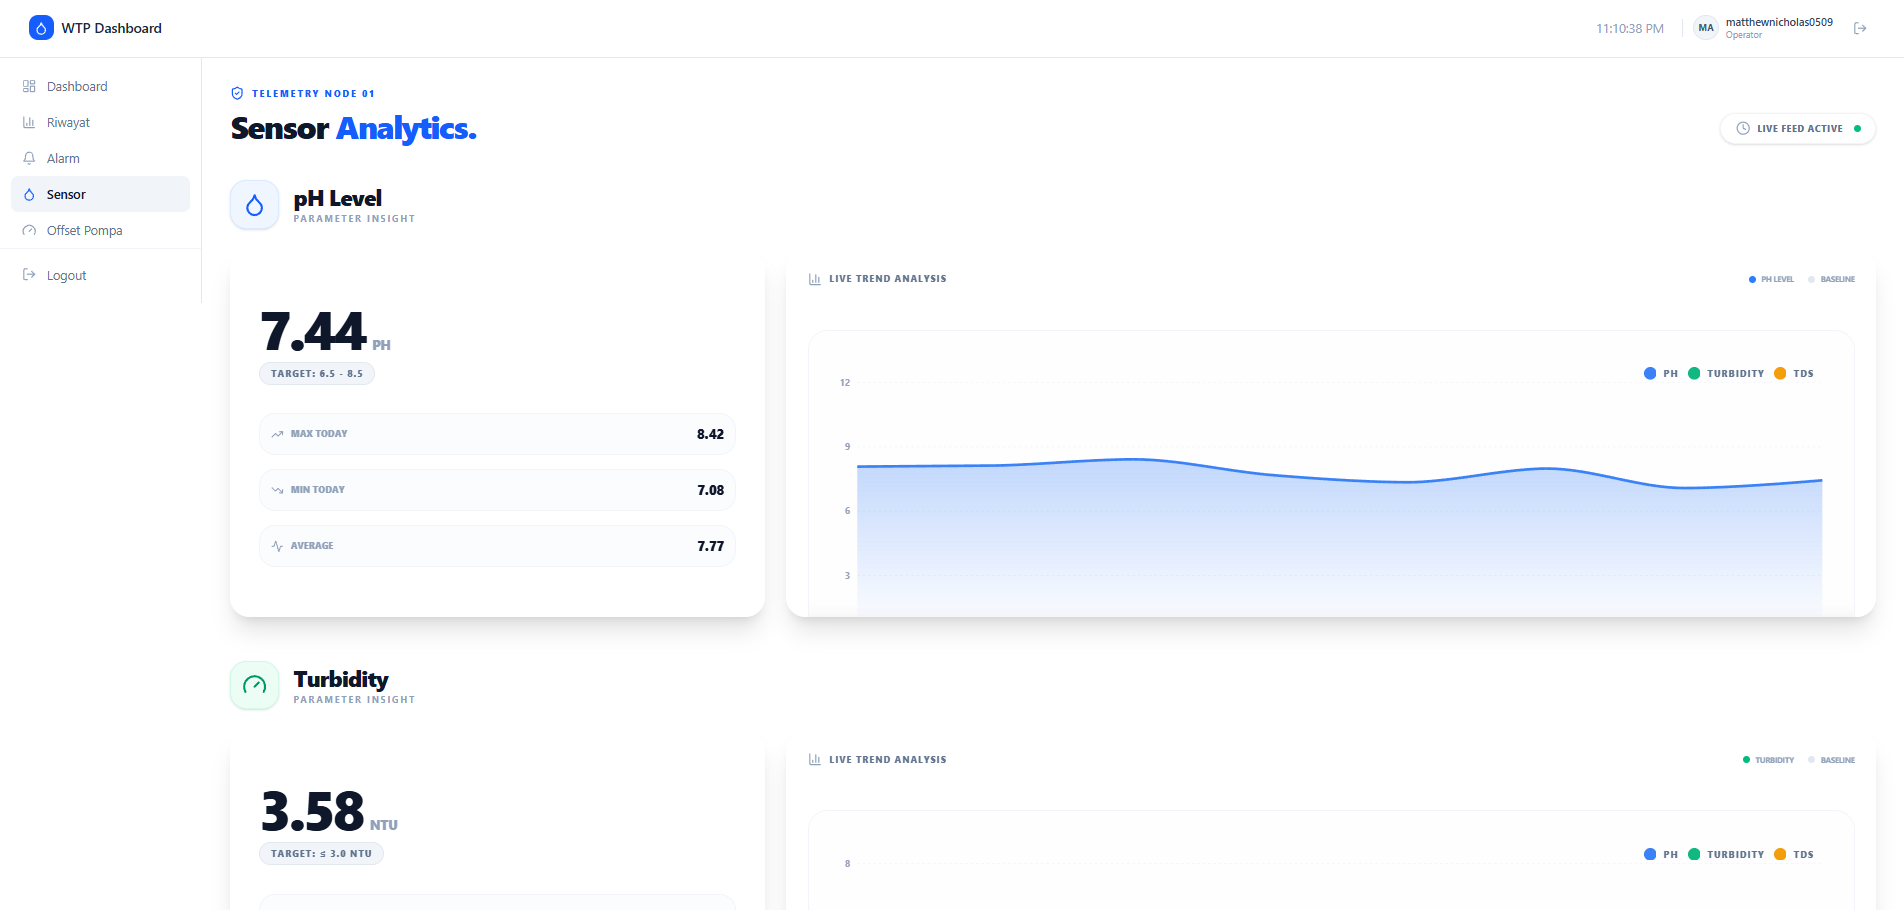
\includegraphics[width=\textwidth]{images/sensor-hifi.png} 
    \caption{Implementasi antarmuka halaman analitik sensor}
    \label{fig:hifi-sensor}
\end{figure}

Berdasarkan Gambar~\ref{fig:hifi-sensor}, komponen-komponen fungsional yang diimplementasikan meliputi:
\begin{enumerate}
    \item \textbf{Indikator Status Telemetri (\textit{Connection Status}):} 
    Di sudut kanan atas halaman, diimplementasikan lencana status dinamis yang menandakan ketersediaan aliran data 
    telemetri terkini (\textbf{LIVE FEED ACTIVE}).

    \item \textbf{Wawasan Parameter (\textit{Parameter Insight}):} 
    Panel di sisi kiri digunakan untuk menampilkan pembacaan sekilas dan ringkasan metrik. Nilai pembacaan 
    terkini (misalnya 7,44 untuk pH) ditampilkan dengan ukuran tipografi terbesar. Di bawahnya, terdapat 
    referensi target operasional (contoh: \texttt{TARGET: 6,5 - 8,5}) sebagai acuan batas aman. Bagian ini juga 
    menyajikan agregasi data harian berupa nilai puncak (\textit{Max Today}), nilai dasar (\textit{Min Today}), 
    dan nilai rata-rata (\textit{Average}).

    \item \textbf{Analisis Tren Langsung (\textit{Live Trend Analysis}):} 
    Panel di sisi kanan memuat grafik area individual untuk memvisualisasikan pergerakan titik 
    data (\textit{data points}) dari satu sensor spesifik. Grafik individual ini mencegah terjadinya penumpukan 
    garis (\textit{overlapping}) seperti yang terjadi pada grafik multivariabelsehingga operator dapat mengamati 
    fluktuasi anomali kecil dengan lebih presisi.
\end{enumerate}

\subsection{Halaman \textit{Offset} Pompa (\textit{Chemical Dosing Control})}
Halaman \textit{Offset} Pompa diimplementasikan sebagai antarmuka intervensi manual yang memberikan 
kewenangan bagi operator untuk menyesuaikan takaran bahan kimia. Antarmuka ini penting untuk 
kondisi operasional di mana algoritma otomasi membutuhkan koreksi dosis karena adanya perubahan pada kualitas air baku. 
Hasil implementasi halaman kendali ini ditunjukkan pada Gambar~\ref{fig:hifi-offset}.

\begin{figure}[htbp]
    \centering
    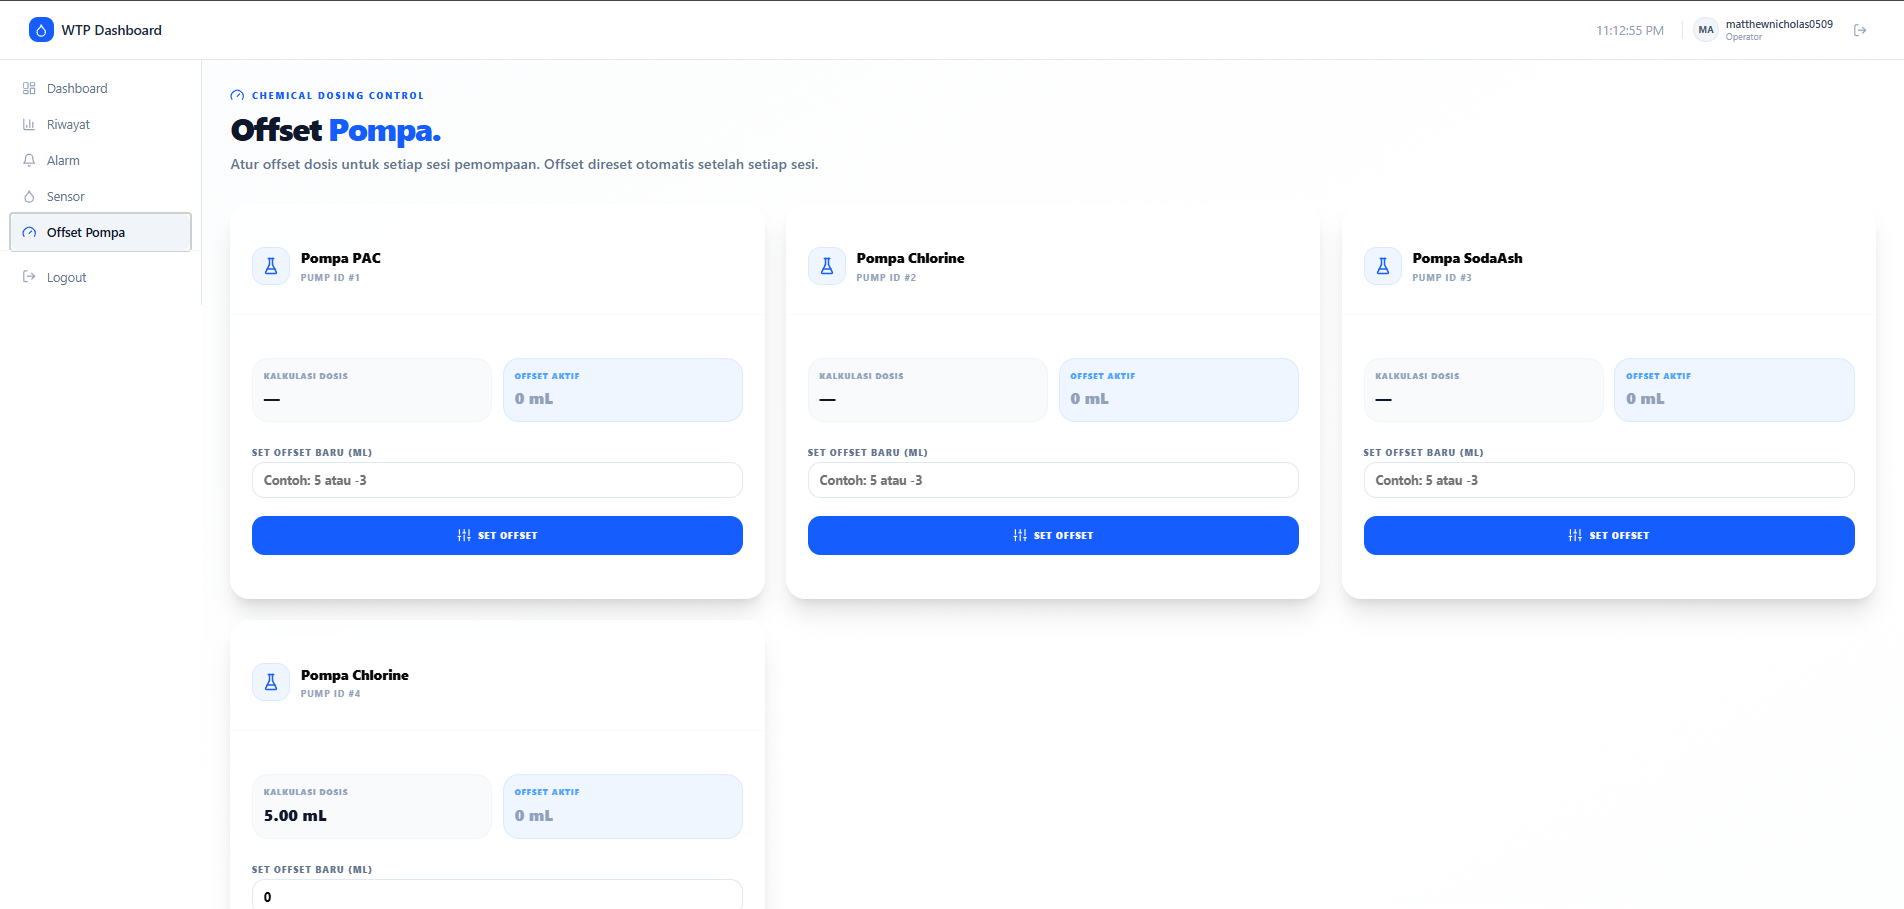
\includegraphics[width=\textwidth]{images/pompa-hifi.png} 
    \caption{Implementasi antarmuka halaman kendali \textit{offset} pompa}
    \label{fig:hifi-offset}
\end{figure}

Berdasarkan Gambar~\ref{fig:hifi-offset}, antarmuka menampilkan tiga panel kendali terpisah yang diletakkan 
secara sejajar untuk masing-masing aktuator bahan kimia, yaitu pompa PAC, pompa kaporit, dan pompa soda ash. 
Setiap panel kendali terdiri dari elemen informasi dan elemen formulir masukan sebagai berikut:
\begin{enumerate}
    \item \textbf{Informasi Status Dosis:} 
    Bagian tengah panel menampilkan metrik \textbf{Kalkulasi Dosis} (takaran yang dihitung oleh algoritma sistem) dan 
    \textbf{\textit{Offset} Aktif} (nilai penyesuaian manual yang saat ini sedang diterapkan). Kedua nilai ini 
    disajikan dalam satuan mililiter (mL).

    \item \textbf{Kolom Masukan Nilai (\textit{Input Field}):} 
    Di bawah informasi status, disediakan sebuah kolom teks tempat operator dapat mengetikkan 
    nilai penyesuaian yang baru (\textbf{Set Offset Baru}). Sesuai dengan petunjuk (\textit{placeholder}) 
    pada kolom masukan tersebut, sistem diimplementasikan untuk menerima baik bilangan positif 
    (untuk menambah takaran dosis) maupun bilangan negatif (untuk mengurangi takaran dosis). Masukan divalidasi 
    di sisi \textit{frontend} sehingga nilai yang bukan berupa angka tidak akan diproses untuk dikirimkan.

    \item \textbf{Tombol Eksekusi Mutasi:} 
    Terdapat tombol utama (\textbf{SET OFFSET}) pada bagian paling bawah 
    setiap panel. Tombol ini berfungsi sebagai pemicu untuk mengirimkan instruksi perubahan dosis ke 
    \textit{backend}. Sesuai dengan aturan operasional yang tercantum di bawah judul halaman, nilai \textit{offset} 
    yang dikirimkan bersifat sementara dan akan diatur ulang (\textit{reset}) secara otomatis oleh sistem setelah 
    satu sesi pemompaan selesai.
\end{enumerate}

\section{Implementasi Autentikasi dan Proteksi Rute}
Seluruh halaman operasional yang telah dijabarkan pada subbab sebelumnya berada di dalam wilayah rute terproteksi. 
Akses menuju halaman-halaman tersebut hanya diberikan kepada operator yang telah berhasil melalui proses autentikasi 
pada halaman \texttt{/login}.

Mekanisme autentikasi diimplementasikan dengan dua alternatif jalur masuk. Jalur pertama adalah autentikasi 
berbasis kredensial lokal, yaitu \textit{username} dan \textit{password}, yang dikirimkan ke \textit{endpoint} 
\texttt{/api/auth/login}. Jalur kedua adalah autentikasi melalui penyedia identitas pihak ketiga berbasis 
protokol OAuth, yang pertukaran tokennya ditangani melalui \textit{endpoint} \texttt{/api/auth/google}.

Setelah autentikasi berhasil, \textit{backend} mengembalikan token akses berbasis \textit{JSON Web Token} (JWT) 
yang selanjutnya digunakan oleh \textit{frontend} sebagai kredensial pada setiap permintaan menuju \textit{endpoint} 
terproteksi. Sesi pengguna dikelola melalui mekanisme penyimpanan token pada sisi klien, sedangkan pembaruan masa 
berlaku sesi ditangani melalui \textit{endpoint} \texttt{/api/auth/refresh}. Ketika operator menutup sesi melalui 
tombol \textit{logout}, \textit{frontend} memanggil \textit{endpoint} \texttt{/api/auth/logout} dan membersihkan 
seluruh token yang tersimpan di sisi klien, kemudian mengarahkan pengguna kembali ke halaman \texttt{/login}.

Proteksi rute diimplementasikan pada tata letak (\textit{layout}) yang membungkus seluruh halaman operasional. 
Setiap kali operator melakukan navigasi menuju rute terproteksi, sistem memvalidasi keberadaan dan masa berlaku 
token sesi. Apabila token tidak ditemukan atau telah kedaluwarsa, akses ditolak dan pengguna dialihkan secara 
otomatis ke halaman \texttt{/login}.

\section{Implementasi Integrasi REST API dan Manajemen \textit{State}}
Integrasi \textit{frontend} dan \textit{backend} diimplementasikan sepenuhnya melalui REST API sesuai 
kontrak yang telah dirancang pada Bab~\ref{chap:perancangan-sistem}. Seluruh permintaan HTTP dilakukan melalui 
sebuah modul klien API terpusat yang bertanggung jawab menyisipkan token autentikasi pada \textit{header} setiap 
permintaan.

Pengelolaan data yang bersumber dari \textit{server} (\textit{server state}) diimplementasikan menggunakan pustaka 
TanStack Query. Setiap kategori data operasional, yaitu ringkasan \textit{dashboard}, telemetri terkini, riwayat 
sensor, daftar alarm, serta status dan \textit{offset} pompa, dipetakan ke dalam kueri tersendiri dengan kunci 
kueri (\textit{query key}) yang unik. Data yang telah diambil disimpan di dalam \textit{cache} dengan jendela masa 
berlaku (\textit{stale time}) yang singkatsehingga permintaan jaringan yang redundan dapat dihindari tanpa 
mengorbankan kemutakhiran informasi.

Untuk data telemetri yang membutuhkan penyajian mendekati waktu nyata, kueri dikonfigurasi dengan interval 
penarikan ulang otomatis (\textit{polling}) sehingga \textit{dashboard} memperbarui dirinya sendiri tanpa 
memerlukan penyegaran halaman oleh operator. Sementara itu, interaksi yang mengubah data pada \textit{backend}, 
yaitu pengakuan alarm dan pengiriman nilai \textit{offset} dosis, diimplementasikan menggunakan fungsi mutasi. 
Setelah mutasi berhasil dieksekusi, sistem memicu invalidasi kueri terkait sehingga data terbaru langsung ditarik 
ulang dari \textit{server} dan antarmuka merefleksikan perubahan tersebut secara konsisten.

Respons mentah dari \textit{backend} tidak langsung dirender, melainkan ditransformasikan terlebih dahulu menjadi 
struktur data yang berorientasi antarmuka, seperti ringkasan kepatuhan, deret data grafik, tabel audit, dan 
indikator status pompa. Seluruh struktur data tersebut didefinisikan menggunakan antarmuka (\textit{interface}) 
TypeScript sesuai kontrak APIsehingga ketidaksesuaian struktur data dapat terdeteksi pada tahap kompilasi.

\section{Implementasi Penanganan Kondisi Data Tidak Normal}
Selain menyajikan data pada kondisi normal, \textit{frontend} diimplementasikan untuk menangani berbagai kondisi 
tidak normal yang dapat terjadi selama proses pengambilan data. Kondisi pemuatan data (\textit{loading}) ditandai 
dengan indikator visual, kondisi data kosong ditandai dengan pesan yang menjelaskan ketiadaan data pada rentang 
yang dipilih, sedangkan kegagalan permintaan (\textit{error}) ditandai dengan pesan galat yang dapat dipahami operator.

Kondisi yang paling kritis adalah data kedaluwarsa (\textit{stale}). Untuk menanganinya, diimplementasikan 
komponen \texttt{DataStaleOverlay} sebagaimana ditunjukkan pada Gambar~\ref{fig:stale}.

\begin{figure}[H]
    \centering
    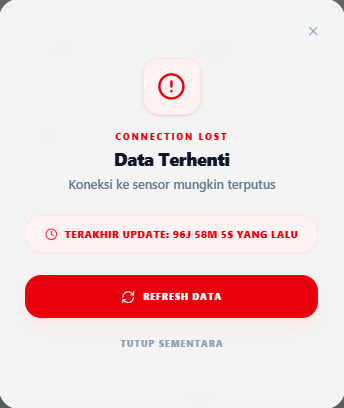
\includegraphics[width=0.5\textwidth]{images/stale.png}
    \caption{Implementasi lapisan peringatan data kedaluwarsa}
    \label{fig:stale}
\end{figure}

Berdasarkan Gambar~\ref{fig:stale}, komponen ini ditampilkan sebagai lapisan modal ketika respons ringkasan 
dari \textit{backend} menandakan bahwa sistem berada dalam kondisi \textit{offline} atau data telemetri terbaru 
tidak tersedia. Lapisan tersebut memuat pernyataan kondisi terputusnya koneksi sensor, penanda usia data yang 
dihitung secara dinamis dari cap waktu pembaruan terakhir, tombol \textbf{Refresh Data} untuk memicu penarikan 
ulang secara manual, serta tautan untuk menutup peringatan sementara. Keberadaan komponen ini mencegah operator 
mengambil keputusan operasional berdasarkan pembacaan yang sudah tidak merepresentasikan kondisi aktual 
instalasi, sekaligus tetap memungkinkan operator mengakses halaman riwayat maupun alarm ketika telemetri terkini 
sedang tidak tersedia.

\section{Implementasi \textit{Progressive Web App} dan \textit{Deployment}}
Aplikasi dikonfigurasi sebagai \textit{Progressive Web App} (PWA) melalui penyediaan berkas \textit{Web App Manifest} 
dan sebuah \textit{service worker}. Konfigurasi ini memungkinkan \textit{dashboard} dipasang langsung pada layar 
beranda perangkat operator, baik pada perangkat \textit{desktop} di ruang kendali maupun perangkat bergerak saat 
operator melakukan patroli lapangan, tanpa memerlukan distribusi melalui toko aplikasi.

Seluruh antarmuka diimplementasikan dengan pendekatan desain responsif sehingga tata letak menyesuaikan diri secara 
proporsional terhadap berbagai ukuran layar. Aplikasi yang telah selesai dibangun kemudian dipasang (\textit{deploy}) 
pada infrastruktur komputasi awan sehingga dapat diakses oleh operator melalui jaringan.